% !TEX root = ../Rulebook.tex

The actual competition contains a set of so-called tests. 
A test is specified in terms of it's purpose and focus, environment features and eventually manipulation objects involved. Further, a concrete specification of the task is given and the rules to be obeyed. 

Each test has different variability dimensions. That is, which objects to be manipulated, how many locations to visit, from which height to grasp etc. These dimensions are described in Section~\ref{sec:TestVariability} whereas in Section~\ref{sec:TestInstances} test instances for \YEAR are defined based on the general test description and instantiation of the variability dimensions. 

%\section{Description of the Test Scenarios}

% !TEX root = ../Rulebook.tex
\newpage
\section{Basic Navigation Test}

\paragraph{Purpose and Focus of the Test}
The purpose of the \iaterm{Basic Navigation Test}{BNT} is to check whether the robots can navigate well in their environment, i.e. in a goal-oriented, autonomous, robust, and safe way.
\par
As the navigation problem is in the focus of robotics research for a long time and many approaches for solving it and its subtasks (like exploration, mapping, self-localization, path planning, motion control, and obstacle avoidance) exist, the focus of this test is to demonstrate that these approaches function properly on the robots used by the teams and in the environment defined by the test.
\par

\paragraph{Scenario Environment}
The arena used for this test contains all elements that affect or support navigation: walls, service areas, places, arena objects, wall markers, and floor markers. In addition, obstacles may be placed in the environment.

\paragraph{Manipulation Objects}
This test does not include any objects for manipulation.
\paragraph{Task}
The robot will be sent a task specification, which is a string containing a series of triples, each of which specifies a place, an orientation, and pause duration. The robot has to move to the places specified in the task string, in the order as specified by the string, orient itself according to the orientation given, cover a place marker, pause its movement for the time in seconds as specified by the pause length, and finally leave the arena to reach the final position.

The task specification consists of:

\begin{itemize}
	\item[--] A destination location, e.g. \texttt{WS01}, \texttt{SH02}, \texttt{CB03} or \texttt{WP12}
	\item[--] An orientation (\texttt{N}, \texttt{S}, \texttt{W}, \texttt{E})
	\item[--] A duration in seconds
\end{itemize}

The duration is always set to 3 seconds in order to make validation easier for the referees.
%
% \subsection{Complexity Options}
%
% \subsubsection{Obstacle complexity (pick one):}
%
% \begin{itemize}
% 	\item Easy obstacles (bonus factor = +0.2): There are up to two obstacles in the arena.
% 	\item Medium obstacles (bonus factor =  +0.4): There are up to three obstacles in the arena and the placement of the obstacles is harder.
% \end{itemize}
%
%
% \subsubsection{Barrier Tape complexity (bonus factor = +0.4):}
% There are up to two barrier tape obstacles in the arena.
%
% \subsubsection{Navigation complexity (pick one):}
%
% \begin{itemize}
% 	\item Easy navigation (bonus factor = + 0.0): The place marker has to be covered in such a way by the robot that at least a part of the black area covered
% 	\item Medium navigation (bonus factor = + 0.1): The place marker has to be covered in such a way by the robot that at least a small part of the black area is covered the orientation must be correct, i.e. the robot must not deviate more than 45 deg.
% 	\item Hard navigation (bonus factor = + 0.2): The place marker has to be fully covered by the robot the orientation must be correct, i.e. the robot must not deviate more than 45 deg.
% \end{itemize}
%
%
\paragraph{Rules}
The following rules have to be obeyed:

\begin{itemize}
\item A single robot is used.
\item The robot has to start from outside the arena, enter it through the arena entrance and leave through the exit.
\item The order in which the teams have to perform will be determined by a draw.
\item After the team's robot enters the arena, it must move to the places given in the task specification and assume the orientation specified after the place. The robot may reach a destination by choosing any path.
\item The robot must visit the places in the order given by the task specification. It is possible to skip a place of the task specification and continue with the next one. In cases where the robot skipped one or multiple places there may be multiple possible matchings between places reached and places specified. In that case for calculating scores the matching is taken which leads to the highest score for the team.
\item A destination is counted as reached when the robot covers the place marker for the number of seconds specified by the break and does not move (very small movement of the wheels is allowed). The orientation must not deviate more than 45 degrees.
\item The run is over when the robot reached the final place or the designated time has expired.
\end{itemize}
%
%
%
% \subsection{Scoring}
%
% \begin{itemize}
% \item The team will receive 50 points for reaching a destination correctly (place and orientation) as given in the task specification and provided it stops for the time specified.
% \item The team receives a penalty of –50 points each time the robot touches an obstacle, a wall, an arena object or a service area (i.e. any contact with the environment).
% \item 50 points are awarded for completing the task specification completely correct, i.e. visiting all destinations from the task specification according to position and orientation (according to the chosen complexity level) and finally leaving the arena.
% \item The reached points of a test will be multiplied with the complexity factor that belongs to the chosen complexity level.
% \end{itemize}


\section{Basic Manipulation Test (BMT)}

\subsection{Purpose and Focus of the Test}
The purpose of the Basic Manipulation Test is to demonstrate basic manipulation capabilities by the robots, like grasping, turning, or placing an object.
\par
The focus is on the manipulation and on demonstrating safe and robust grasping and placing of objects of different size and shape. Therefore, only minimal movement of the robot is required. 
\par
Some minor movement is intentionally designed into this test in order to force the teams to do dynamic assessment of the situation (e.g. estimating positions of manipulation objects, determining grasp positions, etc.) and to avoid that solutions depending on completely known initial situations and well-calibrated systems are possible. 

\subsection{Scenario Environment}
The arena used for this test contains basically all elements as for the Basic Navigation Test. Additionally to environmental elements (walls, service areas, floor markers, etc.), different manipulatable objects will be placed on the service areas. 

\subsection{Manipulation Objects}
The manipulation objects in this test include the objects specified in Table \ref{tab:manipulation_objects}.

\subsection{Task}
A single robot is used. The robot can be placed in an arbitrary starting location by the team. The task consists of a sequence of grasp and place operations, with a small base movement in between. The objective is to move a set of objects from one service area into another. The task is finished once all objects are moved or when the time foreseen for the run ends. 
\par
The task specification consists of: 
\begin{itemize}
	\item The specification of the initial place (e.g. D0, S5, U2)
	\item A source location, given as place (any one)
	\item A destination location, given as place (any one, but nearby the source location)
The specification of a final place for the robot (which does not need to be reached)
\end{itemize}

For now, in the competitions only the line is just as possible configuration:
\par
Line( \textless sequence of objects\textgreater )
\par
Further configurations may be specified in the future. Note, that the pose and orientation of each object in the destination service area is left unspecified and can be chosen by the robot. That means also objects don’t have to be put in a line.

Two examples for a full task specification is as follows:
\begin{itemize}
	\item BMT\textless S6,S6,S7,line(V20,R20,F20\_20\_B),S7\textgreater 
	\item BMT\textless S6,S6,S7,line(F20\_20\_G,F20\_20\_B,M20\_100),S7\textgreater 
\end{itemize}


\subsection{Complexity Options}

\subsubsection{Manipulation Object complexity (pick one):}

\begin{itemize}
\item Choose objects (bonus factor =  0.0): The team can freely choose the manipulation objects.
\item Few objects (bonus factor =  0.2): The team can freely choose a set of five manipulation objects.
\item All objects (bonus factor =  0.5): All manipulations objects can be used.
\end{itemize}


\subsubsection{Decoy Object complexity (pick one):}

\begin{itemize}
\item No decoy objects (bonus factor =  0.0): No decoy objects will be used.
\item Few decoy objects (bonus factor =  0.2): The team can freely choose a set of three manipulation objects, to be used as decoy.
\item All decoy objects (bonus factor =  0.3): All manipulations objects can be used as decoy.
\end{itemize}


\subsubsection{Orientation Complexity (bonus factor = 0.2):}
The manipulation objects can be placed in all orientations.

\subsubsection{Rotation Complexity (bonus factor = 0.2):}
The manipulation objects can be placed in all orientations.

\subsubsection{Position Complexity (bonus factor = 0.2):}
The manipulation objects while be placed by the referees.

\subsection{Rules}
The following rules have to be obeyed:

\begin{itemize}
\item The order in which the teams have to perform will be determined by a draw.
\item A team has a time period of 5 minutes to complete a run.
\item At the beginning of a team’s period, the team will get the task specification. 
\item The team can setup the robot anywhere inside the arena.
\item A manipulation object counts as successfully grasped as defined in Section 5.5.3.
\item A manipulation object counts as successfully placed, if the robot has placed the object into the correct destination service area as described in Section 5.5.4.. 
\item The team has at most 5 minutes to complete the task. The time is stopped when the robot has completed task by placing the last object of the task specification. If a team cannot complete the task within 5 minutes, the run will be stopped after 5 minutes. 
\end{itemize}


\subsection{Scoring}
Points are awarded as follows:

\begin{itemize}
\item 100 points are awarded for successfully grasping a manipulation object that is part of the task specification..
\item 50 points are awarded for successfully placing a manipulation object into the destination service area.
\item - 100 points for grasping a wrong manipulation object.
\item 50 points are awarded for completing the task specification completely correct. 
\item The reached points of a test will be multiplied with a defined complexity factor depending on the previously chosen complexity level.
\end{itemize}



% !TEX root = ../Rulebook.tex

\section{Basic Transportation Test}
\label{sec:Basic Transportation Test}

The \iaterm{Basic Transportation Test}{BTT} targets both navigation and manipulation, aswell as logistical optimization. Objects are initially placed on randomly selected service areas and must be transported to their specific target location.
As their total number now exceeds the inventory size, robots will have to manage their inventory content and optimize their payload. The object pool consists of the complete Basic Object Set.

There are currently two versions of the BTT. 
They gradually introduce more elements of the league to the competition, including the randomness of the used objects, the increase of active Service Areas and them not being next to each other anymore, using different table heights and the placement of physical obstacles.

The following paragraphs summarize the two different levels but DO NOT override the test specification in table \ref{fig:test_specifications_instance}.

\paragraph{BTT1}
\begin{itemize}
\item Four randomly selected objects have to be transported.
\item There will be three active service areas and they are not next to each other.
\item Only tables with a height of 10cm are used. 
\end{itemize}

\paragraph{BTT2}
\begin{itemize}
\item Five randomly selected objects have to be transported.
\item Two randomly selected decoy objects are placed onto one or more randomly selected service areas.
\item There will be four active service areas with each covering one of the four table heights (0, 5, 10, 15 $\si{\centi\meter}$).
\item Physical Obstacles are placed inside the arena (one blocking, one semi-blocking).
\end{itemize}

\newpage
\section{Precision Placement Test}
\label{sec:Precision Placement Test}

\paragraph{Purpose and Focus of the Test}
The purpose of the \iaterm{Precision Placement Test}{PPT} is to assess the robot's ability to grasp and place objects into object-specific cavities. This demands advanced perception abilities (to recognize the correct cavity for each object) and manipulation abilities (to grasp and place the object in such a manner that it fits into the cavity).

\paragraph{Scenario Environment}
The same arena as for the Basic Manipulation Test is used. In case that the arena does not already include a modified service area as shown in Figure \ref{fig:ppt_plattform}, it will be added only for this particular test. The modified service arena includes object-specific cavities as shown in the Figure~\ref{fig:ppt_tiles}. For each object used in the test, there will be one specific cavity. The cavity has the dimension of the object plus a 2 mm offset for each dimension. At most five cavities are used in the test.


\begin{figure} [h!]
\begin{center}
\subfloat[F20\_20]{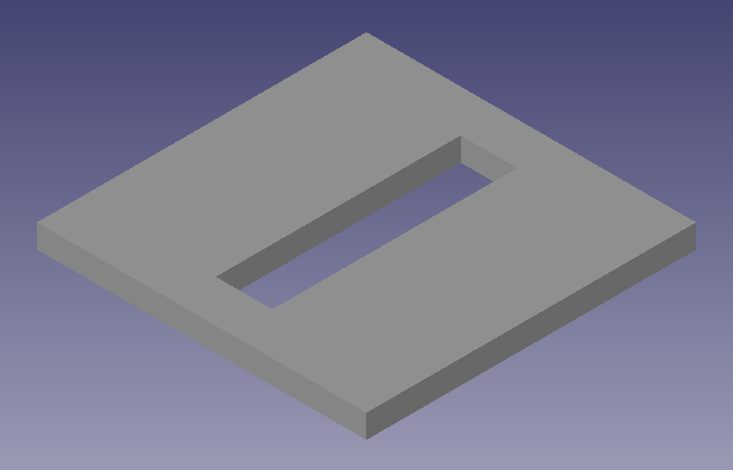
\includegraphics[width = 2cm]{./images/ppt_F20.png}} \hspace{0.1cm}
\subfloat[S40\_40]{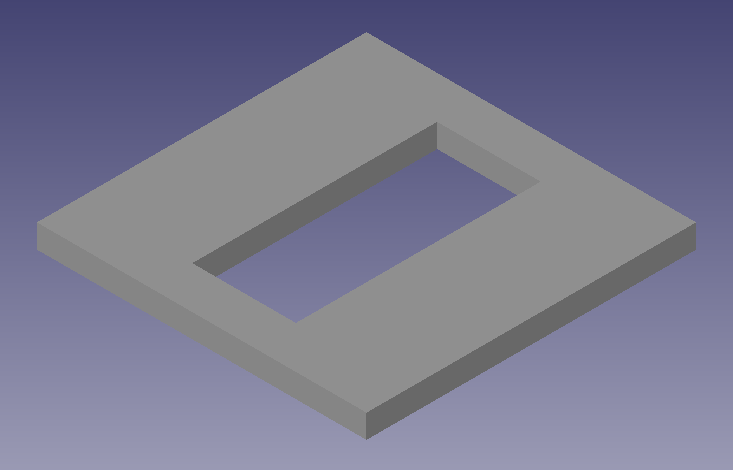
\includegraphics[width = 2cm]{./images/ppt_S40.png}} \hspace{0.1cm} 
\subfloat[M20\_100]{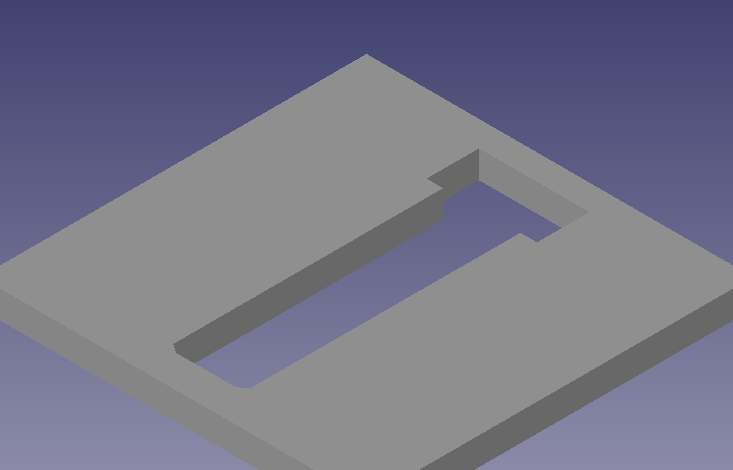
\includegraphics[width = 2cm]{./images/ppt_M20_100.png}}  \hspace{0.1cm}
\subfloat[M20]{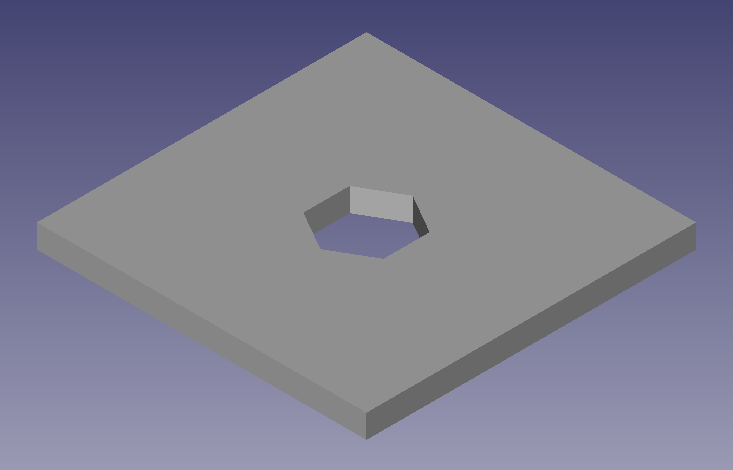
\includegraphics[width = 2cm]{./images/ppt_M20.png}}  \hspace{0.1cm}
\subfloat[M30]{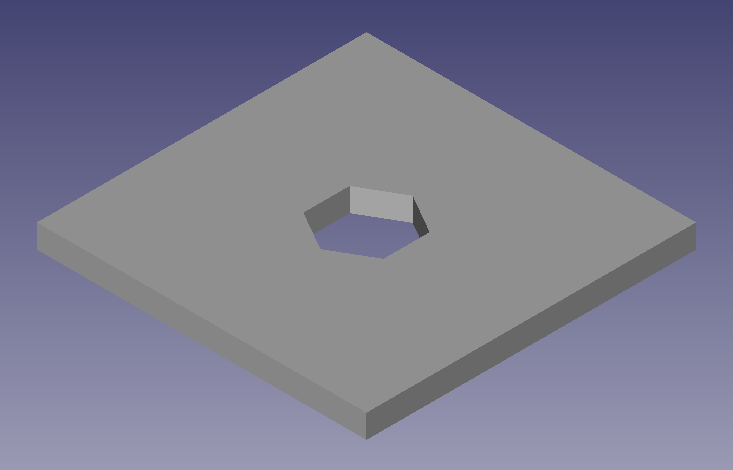
\includegraphics[width = 2cm]{./images/ppt_M30.png}}  \hspace{0.1cm}
\subfloat[R20]{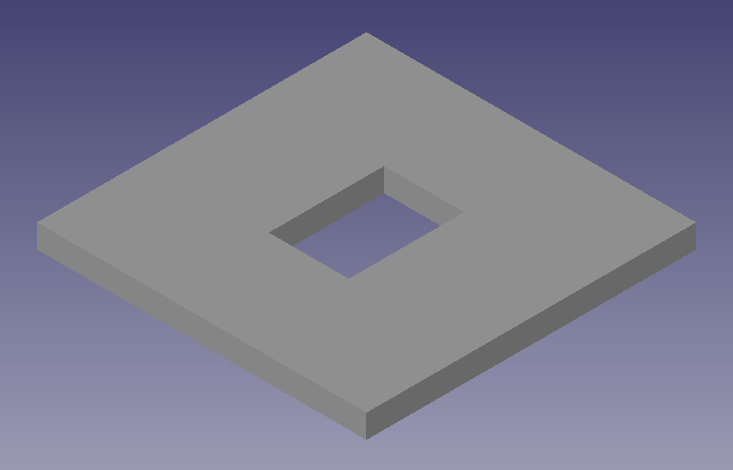
\includegraphics[width = 2cm]{./images/ppt_VR20.png}} \\
\subfloat[F20\_20]{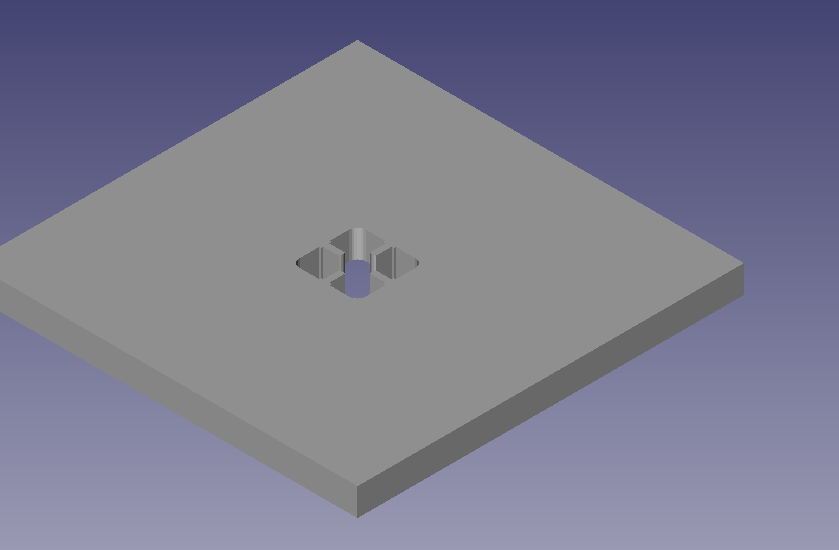
\includegraphics[width = 2cm]{./images/ppt_F20_v.png}}  \hspace{0.1cm}
\subfloat[S40\_40]{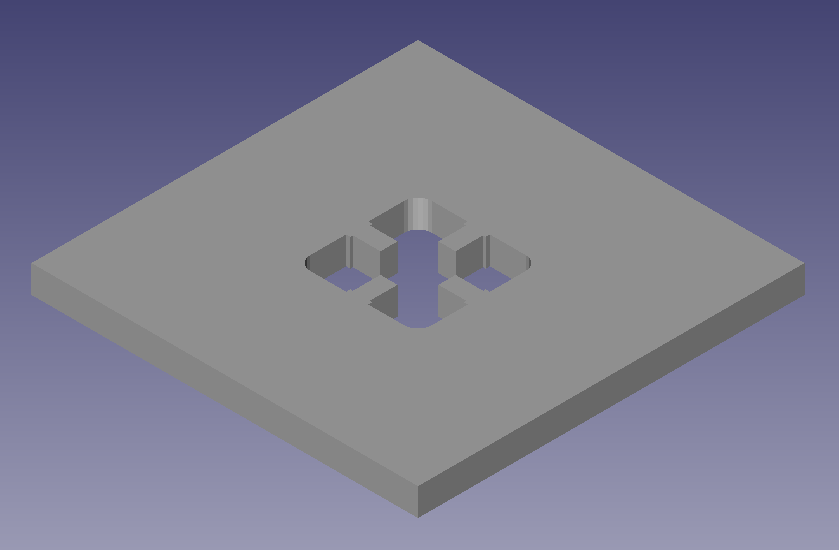
\includegraphics[width = 2cm]{./images/ppt_S40_v.png}}   \hspace{0.1cm}
\subfloat[M20\_100]{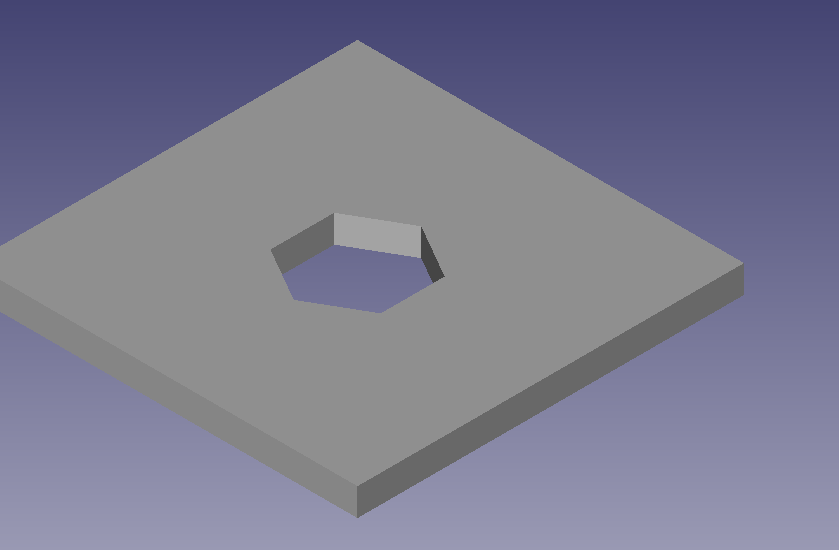
\includegraphics[width = 2cm]{./images/ppt_M20_100_v.png}} \hspace{0.1cm}
\subfloat[M20]{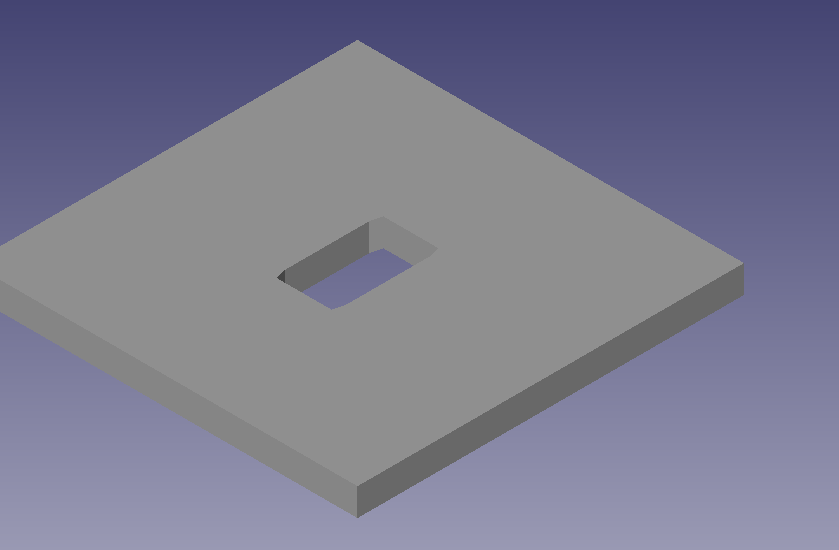
\includegraphics[width = 2cm]{./images/ppt_M20_v.png}}  \hspace{0.1cm}
\subfloat[M30]{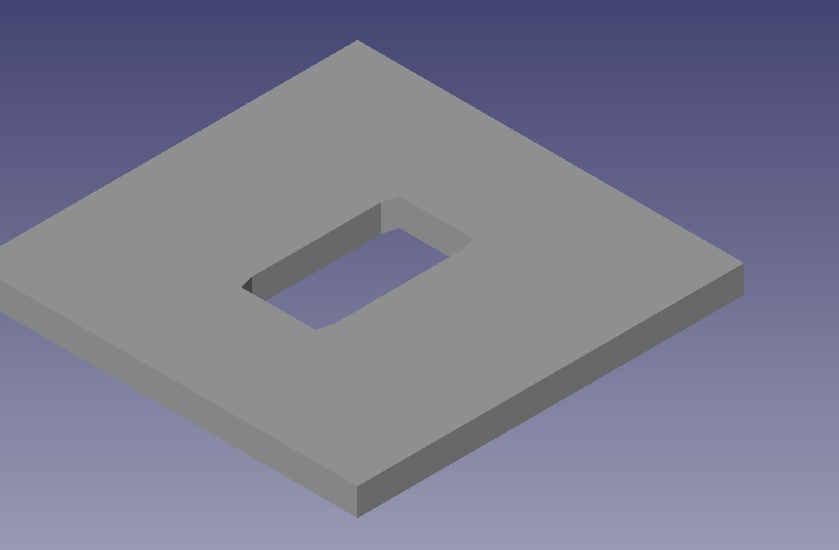
\includegraphics[width = 2cm]{./images/ppt_M30_v.png}}  \hspace{0.1cm}
\subfloat[R20]{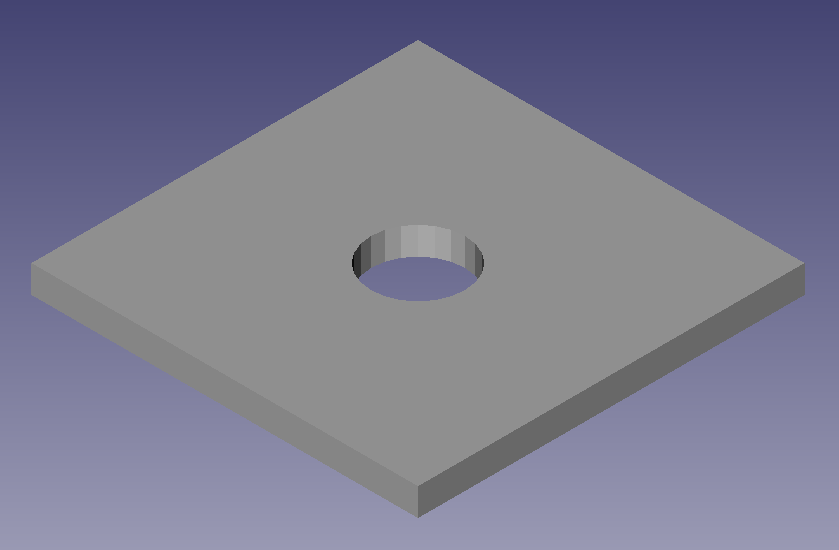
\includegraphics[width = 2cm]{./images/ppt_VR20_v.png}} 
\end{center}
\caption{Illustration of horizontal (top row) and vertical (bottom row) cavities for the different kind of manipulation objects.}
\label{fig:ppt_tiles}
\end{figure}


\paragraph{Manipulation Objects}
The manipulation objects used in this test are defined by the instances described in Table~\ref{tab:Instances}.

\paragraph{Task}
The objective of the task is to pick the objects which are placed on one service area and make a precise placement in the corresponding cavity at the service area with the special PPT platform (an example configuration is illustrated in Figure \ref{fig:ppt_plattform}). 

\begin{figure}
\centering
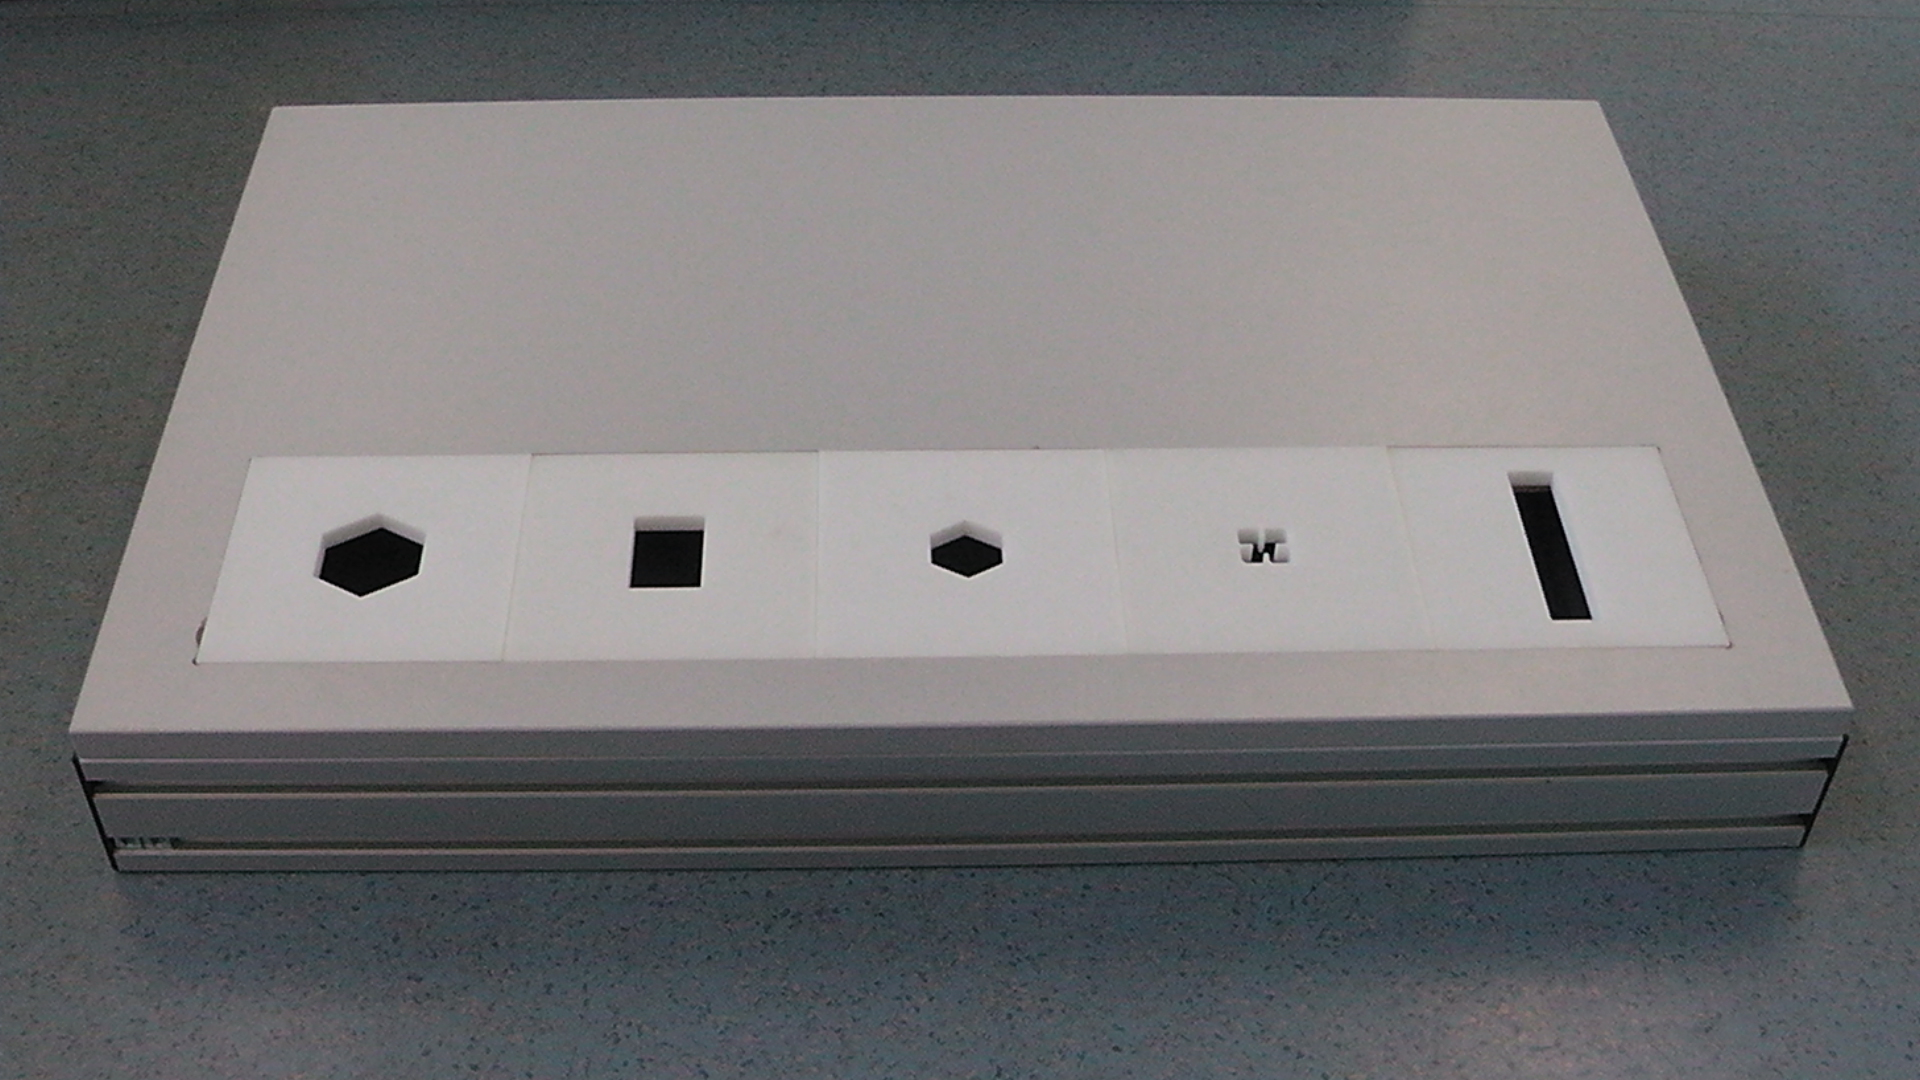
\includegraphics[width=0.6\textwidth ]{./images/ppt_plattform.jpg}
\caption{The PPT platform including five cavity tiles}
\label{fig:ppt_plattform}
\end{figure}

The task consists of multiple grasp and place operations, possibly with base movement in between, which will, however, be short. Note that the placement of the object in the cavity is finished when the object is fallen into the cavity (i.e. at least some part of the object has to touch ground floor underneath the cavity).

%
%\subsection{Complexity Levels}
%
%All Complexity Options from BMT apply.
%
%\subsubsection{PPT Orientation Complexity (bonus factor = 0.2):}
%The cavities can be placed in all orientations.
%\subsubsection{PPT Rotation Complexity (bonus factor = 0.2):}
%The cavities can be placed in all orientations.

\paragraph{Rules}
The following rules have to be obeyed:

\begin{itemize}

\item A single robot is used.
\item The robot has to start from outside the arena and to end in the final.
\item The order in which the teams have to perform will be determined by a draw.
\item The robot will get the task specification from the referee box.
\item A service area counts as successfully reached as defined in Section~\ref{ssec:Navigating}.
%\item A manipulation object counts as successfully grasped as specified in Section~\ref{ssec:GraspingObjects}.
\item An object counts as placed correctly if it fell through the correct cavity and touches the ground beneath. It may happen that an object blocks the cavity for the next object, e.g. by standing upright on the floor. In that case a referee may remove that object (which remains to count as a successful place). If the referee is not able to do so and the robot places another object into the blocked cavity, it counts as a correct placement if it would have been successful without the blocking object.
\item The run is over when the robot reached the final position or the designated time has expired.
\item The score for this test will be calculated as defined in \ref{sec:ScoringAndRanking}.

\end{itemize}

%\subsection{Scoring}
%Points are awarded as follows:
%
%\begin{itemize}
%\item 50 points are awarded for successfully grasping an object.
%\item 100 points are awarded for successfully placing a manipulation object into the correct cavity.
%\item 50 points are awarded if the task specification has been completely fulfilled. The task is considered as fulfilled if all objects have been dropped in the right cavity. The robot does not have to leave the arena.
%\item a penalty of -50 points is given for each object which has been dropped into the wrong cavity
%\item The reached points of a test will be multiplied with a defined complexity factor depending on the previously chosen complexity level.
%\end{itemize}




\newpage
\subsection{Conveyor Belt Test}


\paragraph{Purpose and Focus of the Test}
The purpose of the \iaterm{Conveyor Belt Test}{CBT} is to assess the robot’s ability to manipulate moving objects which are placed on a conveyor belt. The test demands fast perception and manipulation skills in order to pick up objects from an operating conveyor belt.

\paragraph{Scenario Environment}
The same arena as for the Basic Manipulation Test is used (Figures 5.4 and 5.5). In case that the arena does not already include a conveyor belt (see Figure \ref{fig:conveyor_belt}), it will be added only for this particular test.
The OC may choose to use a rotating turntable instead of a linear conveyor belt in order to simplify the setup of the arena. The particular choice shall be announced before the tournament.
An area besides the conveyor belt is left free so that a robot can drive there and grasp the objects from the belt. The other sides might not be accessible, because the device is placed into a corner. 
The conveyor belt should have a wireless mechanism to turn it on. 

\begin{figure} [h!]
\centering
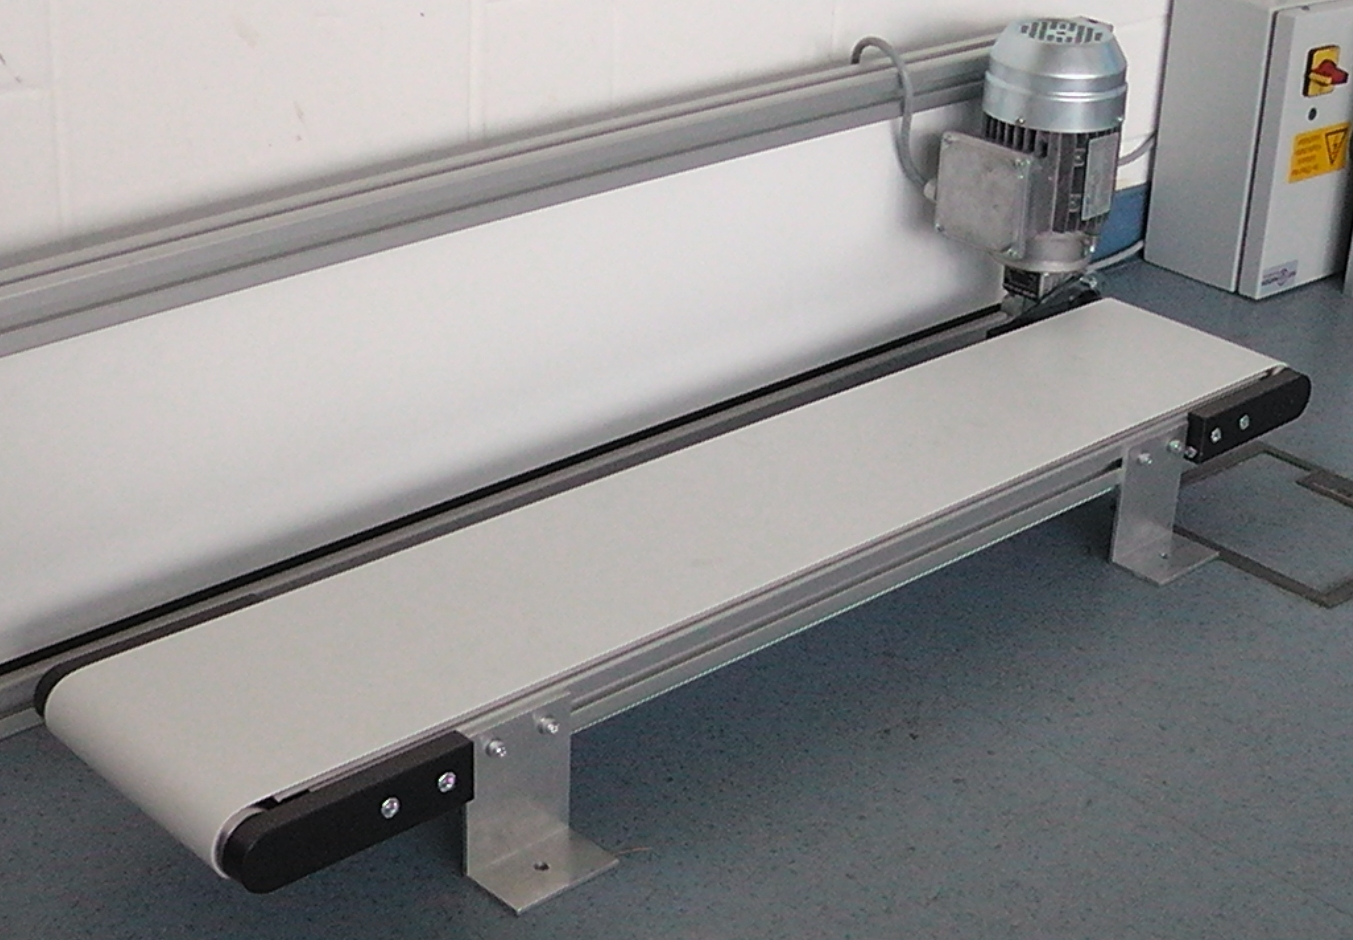
\includegraphics[width=0.5\textwidth ]{../images/conveyor_belt.jpg}
\caption{Illustration of a conveyor belt used in the competition.}
\label{fig:conveyor_belt}
\end{figure}


%\paragraph{Manipulation Objects}
%The same manipulation objects as for the Basic Manipulation Test are used. The team has to choose five objects out of the total object set (see Section 5.5.1). From those five objects, the TC is going to select three objects which will be placed on the conveyor belt. Beside these three objects there will be no other objects on the conveyor belt.

\paragraph{Task}
A single robot is used. The robot is placed by the team in some starting position outside of the arena. Initially the conveyor is switched off (i.e. the belt is not moving) and all objects are put on the belt with a distance between them determined by the TC. The task of the robot is to navigate to the location of the conveyor belt and to grasp all objects from the moving belt before they fall off at the other end of the belt. If a turntable is used, the objects can pass multiple times in front of the robot, until the maximum time for the run is over. The robot is supposed to place the grasped objects on the robot itself. The task is finished once the robot successfully grasped all objects or the foreseen time of the test has been exceeded. 
\par
There are two options to determine when to switch on the conveyor belt:
The robot starts it itself, using the wireless mechanism.
A team member can give a signal to the referees to switch on the conveyor belt.
\par
Teams can decide during the run to give the signal to the referees, e.g. when the robot failed to start it itself. 
\par
The task specification has the following structure:
\par
CBT \textless srv\_area\textgreater
\par
where ‘srv\_area’ is the location of the conveyor belt (e.g. T1)

%\subsection{Complexity Options}
%All Complexity Options from BMT apply.


%\subsubsection{Speed Complexity (pick one):}
%
%\begin{itemize}
%\item low speed (bonus factor = +0.0): The conveyor belt speed will be not more than 0.5 cm/s
%\item medium speed (bonus factor = +02):	The conveyor belt speed will be not more than 0.75 cm/s
%\item high speed (bonus factor = +0.4): The conveyor belt speed will be not more than 0.10 cm/s
%\end{itemize}



\paragraph{Rules}
The following rules have to be obeyed:

\begin{itemize}
\item The order in which the teams have to perform will be determined by a draw.
\item A team has a time period of 10 minutes to complete a run. The time is stopped when the robot has completed the task.
\item At the beginning of a team’s period, the team will get the task specification.
\item The objects are placed on the conveyor before the run starts, for low complexity by the team or for medium and high by a referee..
\item After the team’s robot starts, it must move inside the arena.
\item Either the robot itself starts the conveyor belt, or a team member can give a signal to the referees to switch on the conveyor belt..
\item The objects have to be grasped actively from the moving belt. The robot is not allowed e.g. to wait at the end with a particular basket and collect the falling objects from the end of the conveyor belt. Further, wiping the objects to the side is also not allowed.
\item A manipulation object counts as successfully grasped, if the robot has lifted the object and moved it outside of the area of the conveyor belt as specified in Section 5.5.3 point 2.
\item The team must leave the arena within a minute after completing the task.
\end{itemize}



%
%\subsection{Scoring}
%Points are awarded as follows:
%
%\begin{itemize}
%\item 200 points are awarded for successfully grasping an object from the conveyor belt 
%\item -150 points are given if an object dropped onto the ground, is placed not on the robot itself or dropped from the end of the conveyor..
%\item -100 points are given if the referees had to switch on the belt manually after signalled by a team member, while a working automatic wireless mechanism to switch it on was available.
%\item 50 points are awarded if the task has been fully achieved (when all objects placed on the belt are grasped).
%\end{itemize}


\newpage
\section{Test Variability} \label{sec:TestVariability}

The different optional parameters and configurations for each task are 
mentioned in Section~\ref{sec:ArenaDesign} and \ref{sec:ManipulationTasks}. 
Figure~\ref{fig:complexityTree} summarizes the possible variations and 
emphasizes aspects that may be chosen.

\begin{figure}[ht]
\centering
\tikzset{
  basic/.style  = {draw, rectangle, thin, text width=2cm, 
	                 rounded corners=2pt, align=center},
  root/.style   =  {basic},
  level 2/.style = {basic, sibling distance=45mm},
  level 3/.style = {basic, align=left},
  level 4/.style = {basic, align=left, fill = white!50, node distance = 0.7cm},
	box/.style = {draw, black, dashed}
}

\begin{tikzpicture}[
  font = \footnotesize,
  level 1/.style={sibling distance=70mm},
  edge from parent/.style={->,draw},
  >=latex]

% root of the the initial tree, level 1
\node[root] {Complexities}
% The first level, as children of the initial tree
  child {node[level 2] (c1) {Manipulation}
       child  {node[level 3]  (OBJECTS) {Objects}}
       child {node[level 3]  (GRASPING) {Grasping} }
       child {node[level 3, xshift =-2cm]  (PUTTING) {Putting down} }
	}
  child {node[level 2, xshift=-1cm] (ARENA) {Arena}};

%% OBJECTS
\begin{scope}[every node/.style={level 4,  top color=white!50,bottom color=gray!50,shading angle=45}]
\node [below of = OBJECTS, xshift=15pt, yshift=-20pt] (c11) {@work};
\node [below of = c11] (c12) {Rockin};
\node [below of = c12] (c13) {arbitary};
\node [below of = c13, yshift=-5pt] (c14) {number};
\end{scope}

\node [box, fit = (c11) (c12) (c13)] (BOX) {};
\node at (BOX.north west) [anchor = south west] {Type};

%% GRASPING
\begin{scope}[every node/.style={level 4}]
\node [below of = GRASPING, xshift=28pt, yshift=-20pt] (c21) {0cm};
\node [below of = c21] (c22) {10cm};
\node [below of = c22] (c23) { ??cm};
\node [below of = c23] (c24) { ??cm};
\node [below of = c24, top color=white!50,bottom color=gray!50,shading angle=45, yshift=-18pt] (c25) {Position};
\node [below of = c25, top color=white!50,bottom color=gray!50,shading angle=45] (c26) {Rotation};
\node [below of = c26, top color=white!50,bottom color=gray!50,shading angle=45] (c27) {Orientation};
\node [below of = c27, yshift=-18pt,] (c28) {red};
\node [below of = c28] (c29) { blue};
\end{scope}

\node [box, fit = (c21) (c22) (c23) (c24)] (BOX) {};
\node at (BOX.north west) [anchor = south west] {Height};

\node [box, fit = (c25) (c26) (c27)] (BOX) {};
\node at (BOX.north west) [anchor = south west] {Object Pose};

\node [box, fit = (c28) (c29)] (BOX) {};
\node at (BOX.north west) [anchor = south west] {Container};

%% ARENA
\begin{scope}[every node/.style={level 4}]
\node [below of = ARENA, xshift=15pt, yshift=-20pt] (c31) {Static};
\node [below of = c31] (c32) {Dynamic};
\node [below of = c32, yshift=-5pt] (c33) {Barrier tape};
\end{scope}

\node [box, fit = (c31) (c32)] (BOX) {};
\node at (BOX.north west) [anchor = south west] {Obstacles};

% lines from each level 1 node to every one of its "children"
 \foreach \value in {1,2,3,4}
   \draw[->] (OBJECTS.195) |- (c1\value.west);

 \foreach \value in {1,...,9}
   \draw[->] (GRASPING.195) |- (c2\value.west);
	
 \foreach \value in {1,...,4}
   \draw[->] (PUTTING.345) |- (c2\value.east);

 \foreach \value in {8,...,9}
   \draw[->] (PUTTING.345) |- (c2\value.east);
	
\foreach \value in {1,2,3}
   \draw[->] (ARENA.195) |- (c3\value.west);

\end{tikzpicture}

\caption{Aspects of variability that maybe integrated in a specific instance of a test.}
\label{fig:complexityTree}
\end{figure}


\section{Test Instances \YEAR} \label{sec:TestInstances}
The following instances may occur as an instance of the run. Ranking of the teams will be based on the sum of the achieved points in all the tests.

%\setlength{\tabcolsep}{4.75pt}
\renewcommand{\arraystretch}{1.1}
\newcommand{\R}[2]{
	\begin{turn}{90}
		\begin{minipage}[][1em][c]{#2}
		#1
	  \end{minipage}
	\end{turn}
}

\newcommand{\cir}[1]{\hspace{0.5em}\unitlength1ex\begin{picture}(2.8,2.8)%
\put(0.75,0.75){\circle{2.8}}\put(0.75,0.75){\makebox(0,0){#1}}\end{picture}}
\newcommand{\Y}{{\tiny \CIRCLE}}
\newcolumntype{P}[1]{>{\centering\arraybackslash}p{#1}}

\begin{landscape}
\begin{table}[h!]
 \definecolor{headlineColor}{rgb}{.7,.7,.7}
 \definecolor{sectionColor}{rgb}{.4,.4,.4}
 \centering
 \begin{tabular}{|l|l|l|l*{9}{|P{1cm}}|}
   \hhline{~~~~---------}
   \multicolumn{4}{l|}{ } &  \multicolumn{9}{c|}{ Instances}\\
   \hhline{~~~~---------}
   \multicolumn{4}{l|}{ }          &\cir{1}&\cir{2}&\cir{3}&\cir{4}&\cir{5}&\cir{6}&\cir{7}&\cir{8}&\cir{9}\\
   \multicolumn{4}{r|}{     }        & BNT   & BMT   & BTT1  & BTT2  &  BTT3 &  PPT  &  CBT1   & CBT2 & Final\\
   \hhline{~~~~---------} \hline
    \multirow{27}{0.5cm}{\R{\centering Manipulation }{4cm}}
     & \multirow{7}{0.5cm}{\R{\centering Objects }{0.5cm}}
%    &      \RCAW           & Team     &       &       &       &       &       &       &       &    &    \\ \hhline{~~~----------}
     &      \RCAW           & RefBox   &       &   3   &  5    &   2   &   4   &   3   &   3   & 3  & 5  \\ \hhline{~~-----------}
     &    & RoCKIn          & Team     &       &   2   &       &       &       &       &       &    &    \\ \hhline{~~~----------}
     &    &                 & RefBox   &       &       &       &   3   &   3   &       &       &    & 5  \\ \hhline{~~-----------}
     &    & Decoy           & RefBox   &       &       &  3    &       &   3   &       &       &    & 5   \\ \hhline{~------------}
    %&    & Number          & TC/OC    &       &   5   &  5    &   5   &   7   &   3   &   3   & 3  & 10  \\ 
     \hhline{~------------} \hhline{~------------}
     & \multirow{10}{0.5cm}{\R{\centering Grasping }{2.5cm}}
         & Height           & RefBox   &       & 10 cm & 10 cm &   10 cm    &  0 cm\newline 10 cm\newline 15 cm    &  10 cm & & & 0 cm\newline 5 cm\newline 10 cm\newline 15 cm \\ \hhline{~~-----------}
      &  & Shelf unit       & RefBox   &       &       &       &       &       &       &       &    & 2   \\ \hhline{~~-----------}
%     &  & Position         & Team     &       &       &   \Y  &       &  \Y   &       &       &    &    \\ \hhline{~~~----------}
      &  & Position         & Referee  &       &   \Y  &   \Y  &  \Y   &  \Y   &   \Y  &   \Y  & \Y & \Y  \\ \hhline{~~-----------}
%	  &  & Rotation         & Team     &       &       &       &       &       &       &       &    &    \\ \hhline{~~~----------}
      &  & Rotation         & Referee  &       &   \Y  &   \Y  &  \Y   &  \Y   &   \Y  &   \Y  & \Y & \Y  \\ \hhline{~~-----------}
	  &  & Orientation      & Team     &       &   \Y  &   \Y  &  \Y   &  \Y   &   \Y  &   \Y  & \Y & \Y  \\ \hhline{~~-----------}
%     &  &                  & TC/OC    &       &       &       &       &       &       &       &    &    \\ 
%     &  & Red container    & -        &       &       &       &       &       &       &       &    &    \\
%     &  & Blue container   & -        &       &       &       &       &       &       &       &    &    \\
      &  & Conveyor belt    & RefBox   &       &       &       &       &       &       &   3   &   &     \\ \hhline{~~-----------}
      &  & Rotating turntable& RefBox  &       &       &       &       &       &       &      & 3  & 1   \\ 
      \hhline{~------------} \hhline{~------------}
      & \multirow{4}{0.5cm}{\R{\centering Putting down }{4.5cm}}
         & Height              & RefBox &       & 10 cm &  10 cm & 10 cm    &  0 cm\newline 10 cm\newline 15 cm  &  10 cm & & & 0 cm\newline 5 cm\newline 10 cm\newline 15 cm \\ \hhline{~~-----------}
      &  & Shelf unit          & RefBox &       &       &       &   1   &       &       &       &   & 1   \\ \hhline{~~-----------}
&  & Cavity platform with decoy& RefBox &       &       &       &       &       &  \Y   &       &   & 1   \\ \hhline{~~-----------}
      &  & Red container       & RefBox &       &       &       &   1   &   1   &       &       &   & 1   \\ \hhline{~~-----------}
      &  & Blue container      & RefBox &       &       &       &   1   &   1   &       &       &   & 1   \\ \hhline{~~-----------}
      &  & Rotating turntable  & RefBox &       &       &       &   1   &   1   &       &       &   &    \\ 
    \hhline{-------------} \hhline{-------------}
    \multirow{3}{0.5cm}{\R{\centering Arena }{1.5cm}}
     & \multirow{3}{0.5cm}{\R{\centering }{1.5cm}}
     &     Obstacles (static) & Referee &  2    &       &       &   2   &   2   &       &       &   & 2   \\ \hhline{~~-----------}
%    &   & Dynamic obstacles  & -       &       &       &       &       &       &       &       &   &    \\ \hhline{~~-----------}
     &   & Barrier tape       & Referee &  2    &       &   1   &       &       &       &       &   & 2   \\ \hhline{~~-----------}
     &   & Waypoints          & RefBox  &  9    &       &       &       &       &       &       &   &    \\ 
		\hline \hline
		 \multicolumn{3}{|l|}{Duration} 
		                    & RefBox & 5 min   & 5 min & 5 min  & 5 min & 5 min & 5 min & 5 min & 5 min & 10min \\
		\hline
 \end{tabular}
 \caption{Instances of the \RCAW \YEAR competition (The OC will choose the runs among this selection).}
 \label{tab:Instances}
\end{table}
\end{landscape}


\begin{landscape}
\begin{table}[h!]
 \centering
 \begin{tabular}{|p{5cm}*{9}{|P{1cm}}|}
   \hhline{~---------}
   \multicolumn{1}{l|}{ } &  \multicolumn{9}{c|}{ Instances}\\
   \hhline{~---------}
   \multicolumn{1}{l|}{ }          &\cir{1}&\cir{2}&\cir{3}&\cir{4}&\cir{5}&\cir{6}&\cir{7}&\cir{8}&\cir{9}\\
   \multicolumn{1}{r|}{     }       & BNT    & BMT   & BTT1  & BTT2  &  BTT3 & PPT   &  CBT1 & CBT1 & Finals\\
   \hline\hline
	correct destinations reached    &  50    &       &       &       &       &       &       &      &       \\
    correct object grasping         &        &  100  &  100  & 100   &  100  &       &  300  & 300  &  100 \\ 
    correct object placing          &        &  100  &  100  & 100   &  100  & 300   &       &      &  100  \\ 
	completing whole task           &  50    &  100  &  100  & 100   &  100  & 100   &  100  & 100  &  100  \\ \hline\hline
	maximum attainable points\newline (time bonus not included)   
	                                &  500   & 1100  &  1100 & 1100  & 1500  & 1000  &  1000 & 1000 &  2100 \\ \hline
 \end{tabular}
 \caption{Instances of the \RCAW \YEAR competition (The OC will choose the runs among this selection).}
  \label{tab:InstancePoints}
\end{table}
\end{landscape}
